\documentclass[10pt, aspectratio=169]{beamer}
\usepackage{../beamer_theme_408}
\title{408考研零基础 --- 计算机网络}
\subtitle{4-1 计算机网络概述}
\author{}
\date{}
\begin{document}

\begin{frame}{本节目标}
    \begin{enumerate}
        \item 理解计算机网络的定义
        \item 掌握计算机网络的组成与功能
        \item 熟悉计算机网络的分类
        \item \textbf{掌握三种交换方式{的}原理与区别}
        \item \textbf{理解数据报与虚电路{的}区别}
    \end{enumerate}
\end{frame}

% 使用 subsubsection 或直接用 frame 标题，避免触发 AtBeginSection
\subsubsection{计算机网络的基本概念}
\begin{frame}{计算机网络的定义}
    \textbf{计算机网络}：将\textbf{地理位置不同}的具有\textbf{独立功能}的多个计算机系统，通过通信设备和线路连接起来，由功能完善的\textbf{软件}实现\textbf{资源共享}的系统。\\
    \vspace{0.5em}
    \textbf{要点提炼}：
    \begin{itemize}
        \item \textbf{互连的}：通过通信设备和线路互相连接
        \item \textbf{自治的}：每个计算机拥有独立功能，不依赖于其他计算机
        \item \textbf{集合}：多台计算机组成的整体系统
    \end{itemize}
    \vspace{0.5em}
    \begin{block}{考研提示}
        "互连的、自治的计算机集合"是计算机网络的核心定义。区别于早期的"主机-终端"系统（终端无自治能力）。
    \end{block}
\end{frame}

\begin{frame}{计算机网络的组成 --- 硬件 + 软件}
    \begin{columns}[T]
        \column{0.5\textwidth}
        \textbf{硬件部分}：
        \begin{itemize}
            \item \textbf{主机}（端系统）：服务器、PC等
            \item \textbf{通信链路}：双绞线、光纤、无线电波等
            \item \textbf{交换设备}：路由器、交换机、集线器
        \end{itemize}
        \column{0.5\textwidth}
        \textbf{软件部分}：
        \begin{itemize}
            \item \textbf{协议}：通信双方必须遵守的规则（核心）
            \item \textbf{网络操作系统}：如Windows Server, Linux
            \item \textbf{网络应用软件}：如浏览器、QQ、微信
        \end{itemize}
    \end{columns}
    \vspace{0.5em}
    \begin{block}{协议三要素（常考）}
        \textbf{语法}（格式）、\textbf{语义}（含义/功能）、\textbf{同步}（时序/速度匹配）
    \end{block}
\end{frame}

\begin{frame}{计算机网络的功能}
    \begin{enumerate}
        \item \textbf{数据通信}（最基本功能）：实现信息的传输
        \item \textbf{资源共享}：
        \begin{itemize}
            \item 硬件资源（打印机、高性能服务器）
            \item 软件资源（大型数据库、昂贵的正版软件）
            \item 数据资源（网页内容、在线视频）
        \end{itemize}
        \item \textbf{分布式处理}：将任务分配给多台计算机协作
        \item \textbf{提高可靠性}：某台主机故障，其他主机可替代
        \item \textbf{负载均衡}：均衡分配任务，提高系统效率
    \end{enumerate}
\end{frame}

\subsubsection{计算机网络的分类}
\begin{frame}{按覆盖范围分类}
    \begin{table}
        \begin{tabular}{|c|c|c|c|}
            \hline
            \textbf{类型} & \textbf{全称} & \textbf{范围} & \textbf{关键点} \\ \hline
            \textbf{PAN} & 个人区域网 & $\sim$10m & 蓝牙、Zigbee \\
            \textbf{LAN} & \textbf{局域网} & $\sim$km & \textbf{广播技术}，MAC地址 \\
            \textbf{MAN} & 城域网 & $\sim$100km & 城市骨干网 \\
            \textbf{WAN} & \textbf{广域网} & $\sim$1000km+ & \textbf{交换技术}，IP地址 \\
            \hline
        \end{tabular}
    \end{table}
    \vspace{0.5em}
    \begin{alertblock}{核心区别}
        LAN与WAN的核心区别不仅是距离，更在于\textbf{底层协议和地址机制}（LAN主要靠广播和MAC，WAN主要靠路由和IP）。
    \end{alertblock}
\end{frame}

\begin{frame}{按拓扑结构分类}
    \begin{columns}[T]
        \column{0.2\textwidth}
        \textbf{星型}\\
        易扩展，中心故障全挂
        \column{0.2\textwidth}
        \textbf{总线型}\\
        布线简单，冲突严重
        \column{0.2\textwidth}
        \textbf{环型}\\
        令牌传递，单点故障风险
        \column{0.2\textwidth}
        \textbf{网状}\\
        可靠性极高，成本也高
        \column{0.2\textwidth}
        \textbf{树型}\\
        层次结构，易于管理
    \end{columns}
    \vspace{1em}
    \centering
    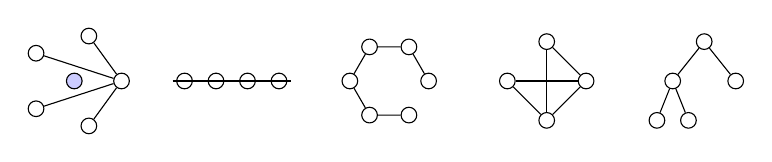
\begin{tikzpicture}[scale=0.5, every node/.style={circle,draw,inner sep=2pt}]
        % Star
        \node (s0) at (0,0) [fill=blue!20] {};
        \foreach \a in {0,72,...,288} \node (s\a) at (\a:1.2) {};
        \foreach \a in {0,72,...,288} \draw (s0)--(s\a);
        
        % Bus
        \begin{scope}[xshift=4cm]
            \draw[thick] (-1.5,0)--(1.5,0);
            \foreach \x in {-1.2,-0.4,0.4,1.2} \node at (\x,0) {};
        \end{scope}
        
        % Ring
        \begin{scope}[xshift=8cm]
            \foreach \a in {0,60,...,300} \node (r\a) at (\a:1) {};
            \draw (r0)--(r60)--(r120)--(r180)--(r240)--(r300)--cycle;
        \end{scope}
        
        % Mesh
        \begin{scope}[xshift=12cm]
            \node (m1) at (0,1) {}; \node (m2) at (1,0) {}; \node (m3) at (0,-1) {}; \node (m4) at (-1,0) {};
            \draw (m1)--(m2)--(m3)--(m4)--cycle; \draw (m1)--(m3) (m2)--(m4);
        \end{scope}
        
        % Tree
        \begin{scope}[xshift=16cm]
            \node (t1) at (0,1) {}; \node (t2) at (-0.8,0) {}; \node (t3) at (0.8,0) {};
            \node (t4) at (-1.2,-1) {}; \node (t5) at (-0.4,-1) {};
            \draw (t1)--(t2) (t1)--(t3) (t2)--(t4) (t2)--(t5);
        \end{scope}
    \end{tikzpicture}
\end{frame}

\section{三种交换方式}

\begin{frame}{电路交换 --- 资源独占}
    \begin{columns}[T]
        \column{0.5\textwidth}
        \textbf{三个阶段}：
        \begin{enumerate}
            \item \textbf{建立连接}：拨号申请
            \item \textbf{数据传输}：占用专用通路
            \item \textbf{释放连接}：拆除通路
        \end{enumerate}
        \column{0.5\textwidth}
        \textbf{优缺点}：
        \begin{itemize}
            \item[\color{green!70!black}$\checkmark$] 实时性极佳，无冲突
            \item[\color{red!70!black}$\times$] \textbf{资源利用率极低}
            \item[\color{red!70!black}$\times$] 建立连接时间长
        \end{itemize}
    \end{columns}
    \vspace{1em}
    \begin{exampleblock}{形象类比}
        \textbf{打电话}：你接通电话后就算不说话，这条线别人也用不了。
    \end{exampleblock}
\end{frame}

\begin{frame}{报文交换 --- 存储转发}
    \begin{itemize}
        \item \textbf{过程}：源节点将整个报文发送给相邻节点，相邻节点收到并\textbf{全部存储}后，再转发给下一个节点。
        \item \textbf{优点}：动态分配带宽，提高利用率。
        \item \textbf{缺点}：时延大，对中间节点存储空间要求高。
    \end{itemize}
    \vspace{1em}
    \begin{exampleblock}{形象类比}
        \textbf{寄信}：你写一封厚厚的信丢进邮箱，邮局收齐后整袋转运。
    \end{exampleblock}
\end{frame}

\begin{frame}{分组交换 --- 现代网络基础}
    \begin{itemize}
        \item \textbf{核心思想}：将大报文切割为若干小的\textbf{分组}（Packet）。
        \item \textbf{机制}：存储转发。但因为分组小，存储时间短，时延大大降低。
        \item \textbf{分类}：
        \begin{enumerate}
            \item \textbf{数据报}（Datagram）：无连接，分组独立选路（互联网主流）。
            \item \textbf{虚电路}（Virtual Circuit）：逻辑连接，分组走固定路径。
        \end{enumerate}
    \end{itemize}
    \vspace{0.5em}
    \begin{exampleblock}{形象类比}
        \textbf{发快递}：大件家具拆成几个小包裹，每个包裹都有面单，独立运输。
    \end{exampleblock}
\end{frame}

\begin{frame}{分组交换详解：数据报 vs 虚电路}
    \begin{table}
        \small
        \begin{tabular}{|l|c|c|}
            \hline
            \textbf{特性} & \textbf{数据报方式} & \textbf{虚电路方式} \\ \hline
            连接建立 & \textbf{不需要} & \textbf{需要} \\
            分组路径 & 独立选择（可能乱序） & 固定路径（按序到达） \\
            故障响应 & 自动绕行 & 虚电路断开需重连 \\
            适用场景 & 互联网、非实时应用 & ATM、对质量有要求的场景 \\
            \hline
        \end{tabular}
    \end{table}
    \vspace{0.5em}
    \begin{block}{重要结论}
        TCP协议虽然提供"面向连接"的服务，但它是工作在\textbf{运输层}的，其底层的\textbf{网络层}仍然使用的是无连接的\textbf{数据报}分组交换。
    \end{block}
\end{frame}

\begin{frame}{三种交换方式总结对比}
    \centering
    \begin{tikzpicture}[scale=0.8, >=stealth]
        % Draw time lines
        \draw[thick,->] (0,4) -- (0,0) node[below] {主机A};
        \draw[thick,->] (4,4) -- (4,0) node[below] {交换机};
        \draw[thick,->] (8,4) -- (8,0) node[below] {主机B};
        \node at (-1,2) {时间 $t$};
        
        % Simplified illustration for Grouping (just symbolic)
        \node at (4,4.5) {\textbf{存储转发示意 (分组交换)}};
        \draw[blue, thick] (0,3.5) -- (4,3.0);
        \draw[blue, thick] (0,3.3) -- (4,2.8);
        \draw[blue, thick] (4,3.0) -- (8,2.5);
        \draw[blue, thick] (4,2.8) -- (8,2.3);
    \end{tikzpicture}
    \vspace{0.5em}
    \begin{enumerate}
        \item \textbf{电路交换}：建立连接 $\rightarrow$ 传输 $\rightarrow$ 释放。适合海量持续数据。
        \item \textbf{报文交换}：整个报文存储转发。已基本被淘汰。
        \item \textbf{分组交换}：小块数据存储转发。灵活性最高，时延最低。
    \end{enumerate}
\end{frame}

\begin{frame}{[例题] 电路交换与分组交换的时延比较}
    \textbf{题目}：传送1MB数据，链路速率1Mbps。电路交换建立时间100ms。分组交换分组长1000B（含头20B），共经3段链路（2个路由器）。求总时延（忽略传播/处理时延）。\\
    \vspace{0.5em}
    \textbf{解析}：
    \begin{enumerate}
        \item \textbf{电路交换}：$T = 100\text{ms} + \frac{1\text{MB} \times 8}{1\text{Mbps}} = 100\text{ms} + 8.3886\text{s} \approx 8.49\text{s}$
        \item \textbf{分组交换}：
        \begin{itemize}
            \item 分组数 $k = \frac{1\text{MB}}{1000-20\text{B}} \approx 1049$
            \item 发送时延 $t_s = \frac{1000 \times 8}{10^6} = 8\text{ms}$
            \item 最后一个分组到达需经过路由器转发：$(1049-1) \times 8\text{ms} + 3 \times 8\text{ms} \approx 8.416\text{s}$
        \end{itemize}
    \end{enumerate}
    \textbf{结论}：对于突发数据，分组交换通常更高效。
\end{frame}

\begin{frame}{本节总结}
    \begin{enumerate}
        \item \textbf{核心定义}：互连、自治、资源共享
        \item \textbf{分类}：PAN, LAN(MAC), MAN, WAN(IP)
        \item \textbf{拓扑}：星型、总线、环型、网状、树型
        \item \textbf{交换方式}：
        \begin{itemize}
            \item 电路交换（专线，效率低）
            \item 报文交换（整报存储）
            \item \textbf{分组交换}（小块转发，主流）
        \end{itemize}
        \item \textbf{数据报 vs 虚电路}：无连接与面向逻辑连接
    \end{enumerate}
\end{frame}

\end{document}
